\chapter{Kernels}
\label{h:kernels} 
In dit hoofdstuk gaan we de kernels bespreken die we ontwikkeld hebben. We beperken ons tot derde-orde tensoren.
We gaan ons ook enkel focussen op kernels voor de grafische kaart. Omdat we de kernels geoptimaliseerd zijn voor

\section{Geschiktheid bepalen}
Voor we een kernel ontwikkelen gaan we eerst kijken of de snelheid van het algoritme beperkt wordt door het geheugen of de rekenkracht. Hiervoor voeren we twee nieuwe begrippen in: de rekenverhouding en het kantelpunt.

\subsection{Rekenverhouding en kantelpunt}
De verhouding tussen het aantal rekenoperaties en het aantal getallen dat we lezen en schrijven noemen we de rekenverhouding. De rekenverhouding waarbij het geheugen en de rekeneenheden even snel werken noemen we het kantelpunt. In enkele precisie kunnen we 2,703 Tflop(sp)/s verwerken en het geheugen heeft een bandbreedte van 176 GB/s. Met deze gegevens kunnen we het kantelpunt berekenen voor berekeningen met enkele precisie:
\[
	\frac{2703 \text{Gflop(sp)/s} \times 4 \text{B/float}}
         {176 \text{GB/s}}										= 61,43 \text{flop(sp)/float}
\]
We kunnen dezelfde berekening ook doen voor dubbele precisie. De GPU kan in dubbele precisie 675,75Gflop(dp)/s verwerken.
\[
	\frac{675,75 \text{Gflop(dp)/s} \times 8 \text{B/double}}
         {176 \text{GB/s}}										= 30,71 \text{flop(dp)/double}
\]
Voor beide CPU's op Falcon liggen de kantelpunten op:
\[
	\frac{230,4 \text{Gflop(sp)/s} \times 4 \text{B/float}}
         {64 \text{GB/s}}										= 14,4 \text{flop(sp)/float}
\]
\[
	\frac{115,2 \text{Gflop(dp)/s} \times 8 \text{B/double}}
         {64 \text{GB/s}}										= 14,4 \text{flop(dp)/double}                                    
\]

Wanneer de rekenverhouding hoger is dan het kantelpunt, wordt de uitvoeringstijd van het algoritme beperkt door de rekenkracht. Hoe hoger de rekenverhouding, hoe gunstiger het is om algoritme op de grafische kaart uit te voeren. Wanneer de rekenverhouding kleiner is dan het kantelpunt zijn er niet genoeg rekenoperaties om de rekeneenheden bezig te houden en zal het algoritme beperkt worden door de snelheid van het geheugen. Zie figuur \ref{kantelpunt} voor rekenkracht en bandbreedte voor een gegeven rekenverhouding.

\begin{figure}
\centering
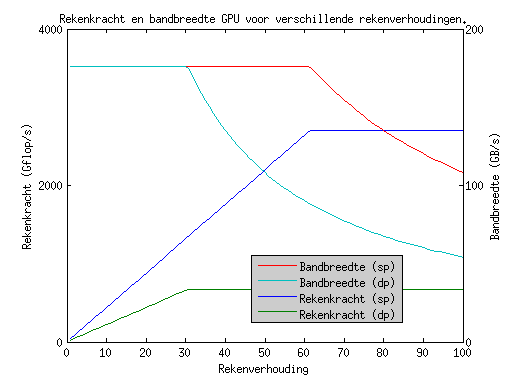
\includegraphics{kantelpunt}
\caption{\label{kantelpunt}De rekenkracht en de bandbreedte van de GPU voor verschillende rekenverhoudingen. Dit zowel voor dubbele als enkele precisie. Merk op dat de curves knikken bij de kantelpunten 61,43 flop(sp)/float en 30,71 flop(dp)/double.}
\end{figure}

Stel dat de rekenverhouding slechts de helft is van het kantelpunt en dat we in dubbele precisie werken. Dit betekent dat de rekeneenheden maar aan de helft van hun snelheid kunnen werken en dat het geheugen aan volle snelheid kan werken. Omdat we maar de helft van de rekenkracht kunnen gebruiken, kunnen we slechts 338 Gflop(dp)/s verwerken.

Wanneer de rekenverhouding gelijk is aan 14,4 flop(dp)/double (het kantelpunt van de CPU) halen de CPU's 115,2 Gflop(dp)/s en haalt de GPU 316,5 Gflop(dp)/s. (675,75 Gflop(dp)/s $\times$ (14,4 flop(dp)/double $\div$ 30,71 flop(dp)/double)) Wanneer de rekenverhouding nog lager is, blijft de verhouding tussen de rekenkracht van de CPU's en de rekenkracht van de GPU constant.

Men zou dus kunnen denken dat de GPU altijd superieur is aan de CPU's. Maar dan vergeet men dat er een grote traagheid is op het geheugen van de GPU en dat er genoeg wavefronten moeten zijn om de piek-performantie van de GPU te kunnen bereiken. Dit zal niet altijd het geval zijn. Een eenvoudig voorbeeld hiervan is het berekenen van een recursief gedefinieerde reeks.

\subsection{Berekenen van de flop's}
Sommige drijvendekomma-operaties vragen meer rekenkracht van de GPU dan andere operaties. Tijdens het berekenen van de flop's gaan we hier rekening mee houden. Tabel \ref{flopTabel} geeft een overzicht van het aantal flops die we aan een operatie toekennen.

\begin{table}
	\centering
	\begin{tabular}{|l|c|c|}
		\hline
		Operatie	& \begin{tabular}{c} Aantal per\\cyclus per PE \end{tabular} & flop's \\
		\hline
		ADD(sp)	&	4	&	2\\
		MUL(sp)	&	4	&	2\\
		MAD(sp)	&	4	&	2\\
		\hline
		ADD(dp)	&	2	&	1\\
		MUL(dp)	&	1	&	2\\
		MAD(dp)	&	1	&	2\\
		\hline
	\end{tabular}
	\caption{\label{flopTabel} Deze tabel geeft het aantal operaties dat een processing-element kan uitvoeren in \'e\'en cyclus. (Bron: handleiding AMD\cite[p.~6-41]{amd}) Hieruit worden de gewichten bepaald voor het berekenen van de flop's.}
\end{table}

We hebben de tabel als volgt opgesteld. Eerst hebben we de eerste kolom ingevuld. Deze informatie komt uit de handleiding van AMD\cite[p.~6-41]{amd}. Daarna hebben we de flop's voor een multiply-add (MAD) gelijksteld aan twee. Vervolgens vullen we de rest van tweede kolom aan met de MAD als referentie.

Bij het toewijzen van flop's moeten we echter opletten. Als we de MAD negeren zullen we onterecht extra flop's aanrekenen. Stel dat we het aantal flops willen berekenen van volgende bewerking: $a = (b*c*d) + e$. Als we de MAD negeren komen we uit op zes flop. (zowel voor dubbele als voor enkele precisie) We zullen rekening houden met de MAD door de som van de MAD gelijk te stellen aan 0 flop's. In het voorgaande voorbeeld rekenen we dus als volgt: \\MUL + MUL + ADD $\rightarrow$ 2 + 2 + 0 (MAD) = 4 flop. We zullen ook steeds aangeven wanneer we de som niet meerekenen vanwege de MAD.

%\todo{enkel 3D}
%\todo{nodige verhouding}

%\todo{flop uitleggen}
%\todo{in stapjes bla bla}

\section{Geschiktheid $f(\T, \mUUU)$}
\label{h:kernels:f:haal}

We herhalen nog eens de functie die we willen parallelliseren:
\begin{align*}
	f &= \sum_{i = 1}^I \sum_{j = 1}^I \sum_{k = 1}^I \left( \left( \sum_{r=1}^{R} u^{(1)}_{i r} u^{(2)}_{j r} u^{(3)}_{k r} \right) - t_{ijk}\right)^2 \\
\end{align*}

We moeten eerst nagaan of $f(\T, \mUUU)$ geschikt is om te parallelliseren. Hiervoor moeten we de rekenverhouding berekenen:\\
\begin{tabular}{|r l|c| c|c|}
\hline
					&							& flop(sp)			& flop(dp) 			& \# geh. aanvragen	\\
\hline
$a_{ij r} $	&$= u^{(1)}_{i r} \cdot%
u^{(2)}_{j r}$									& $2 R \cdot I^2$	& $2 R \cdot I^2$	&	$2RI$			\\
$a_{ijk r} $&$= a_{ij r} \cdot u^{(3)}_{k r}$	& $2 R \cdot I^3$	& $2 R \cdot I^3$	&	$RI$			\\
$a_{ijk} $	&$= \sum_{r=1}^{R} a_{ijk r}$		& 0 (MAD)			& 0 (MAD)			&	$0$				\\
\hline
$a_{ijk} $	&$= a_{ijk}  - t_{ijk}$				& 0 (MAD)			& 0 (MAD)			&	$I^3$			\\
$a_{ijk} $	&$= a_{ijk} a_{ijk}$				& $2 I^3$			& $2 I^3$			&	0				\\
$f $		&$= \sum a_{ijk}$					& 0 (MAD)			& 0 (MAD)			&	0				\\
\hline
\end{tabular}

De totale rekenverhouding is gelijk aan:

\begin{align*}
    & \frac{2R (I^2 + I^3) + 2I^3}{3RI + I^3}\\
\end{align*}

\begin{figure}
\centering
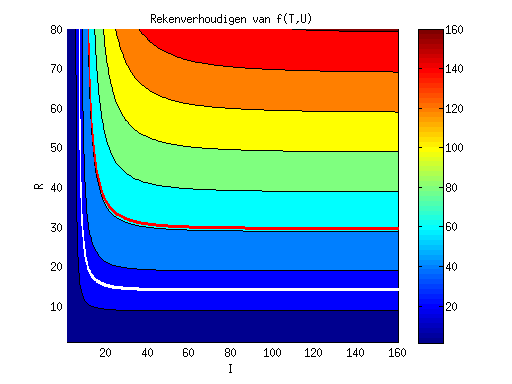
\includegraphics{haalF}
\caption{\label{haalF}De rekenverhoudingen van $f(\T, \mUUU)$. Het kantelpunt voor berekeningen met enkele precisie is getekend met een rode lijn. Het kantelpunt voor berekeningen met dubbele precisie is getekend met een witte lijn.}
\end{figure}

Wanneer we de rekenverhoudingen plotten (figuur \ref{haalF}), zien we dat de kantelpunten convergeren naar $R = 30$ en $R = 14$ wanneer $I$ groter wordt. We kunnen deze waardes van R ook eenvoudig afleiden uit de formule:
\begin{align*}
    61,43 =& \lim_{I \to \infty} \frac{2R (I^2 + I^3) + 2I^3}{3RI + I^3} &
    30,71 =& \lim_{I \to \infty} \frac{2R (I^2 + I^3) + 2I^3}{3RI + I^3}\\
    %
    61,43 =& \frac{2RI^3 + 2I^3}{I^3} &
    30,71 =& \frac{2RI^3 + 2I^3}{I^3}\\
    %
    61,43 =& 2R + 2 &
    30,71 =& 2R + 2\\
    %
    R =& 29,72 &
    R =& 14,36\\
\end{align*}

Uit figuur \ref{haalF} leiden we af dat de rekenkracht van de GPU ten volle kunnen benutten als $R$ en $I$ groot genoeg zijn en als we $f(\T, \mUUU)$ effici\"ent berekenen. Het is de moeite waard om dit algoritme op de grafische kaart uit te voeren.

%De rekenverhouding in ($R$=15, $I$=40) is gelijk aan 31,85 flop(dp)/s.
%De rekenverhouding in ($R$=31, $I$=40) is gelijk aan 61,95 flop(sp)/s.
%Deze rekenverhoudingen liggen juist boven de kantelpunten. Merk ook op dat de rangen slechts een paar eenheden boven de convergentierangen liggen. We besluiten dat $f(\T, \mUUU)$ voor enkele precisie zeker geschikt is om te parallelliseren wanneer $I$ groter is dan 40 en R groter is dan 31. Voor dubbele precisie moet $I$ boven 40 liggen en $R$ boven 15.

%Wanneer we dat evalueren voor $I = R = 50$, dan is de verhouding gelijk aan 98,11. Dit is ruim voldoende. We besluiten dat voor bepaalde realistische probleemgroottes het geheugen de rekenkracht niet zal beperken. Het is dus zeker de moeite om het algoritme te parallelliseren.

%\section{Indelen NDRange}
\section{Float4x4x4 kernel}
De kernel is een combinatie van vele optimalisaties en beslissingen. Om de lezer niet te overweldigen zullen we de kernel stap voor stap opbouwen. Bij elke stap zullen we ook meten hoeveel winst we met elke stap maken. We zullen de winst meten door de tijd te meten die de kernel nodig heeft om uit te voeren. We meten in de volgende vier punten:
\begin{itemize}
    \item I = 16, R = 16
    \item I = 16, R = 6000
    \item I = 320, R = 16
    \item I = 320, R = 6000
\end{itemize}
Door punten de punten zo te kiezen, kunnen we meer inzicht krijgen in de impact van de optimalisatie bij verschillende waardes van R in I.


\subsection{Een eerste kernel}
Zie \ref{codeFloat} voor de volledige broncode van de eerste versie van de kernel.
We gaan nu elk onderdeel van deze kernel toelichten.

\subsubsection{Voor de R-lus}
De eerste lijnen vorm de declaratie van de kernel. De declaratie bestaat uit de volgende elementen:

\begin{tabular}{l p{9cm}}
    \code{\_\_kernel void Kernel} & De kernel noemen we ``Kernel''\\
	\code{\_\_global const float* T} & Het stukje globaal geheugen waarin we de tensor \TT{} opslaan.\\
	\code{\_\_global const float* U1} & De eerste factormatrix \UU{1}.\\
	\code{const int R} & De rang van de ontbinding.\\
	\code{\_\_global float* sum} & Het stukje globaal geheugen waar elke work-group zijn stuk van de som naar wegschrijft. (Zie \ref{calcSum})\\
	\code{const int I1} & Het aantal work-items in mode \'e\'en.\\
	\code{\_\_local float* l} & Het stukje van het lokaal geheugen waar elk work-item zijn stuk van de som naar wegschrijft. (Zie \ref{calcSum})\\
\end{tabular}

In de volgende twee lijnen declarenen we een tijdelijke variabele (\code{float temp;}) en een stukje registergeheugen waar we \'e\'en element van \CC{} in opslaan. (\code{float c = 0;}) We gebruiken \code{c} ook om het element van \CC{} in op te bouwen.

\subsubsection{Itereren over R}
Stel dat we $r$ indelen volgens een dimensie van de NDRange. Dan moeten we twee kernels schrijven. Een eerste die $u^{(1)}_{i r} u^{(2)}_{j r} u^{(3)}_{k r}$ uitrekent en een tweede die de rest van de berekeningen doet. Door deze opsplitsing ontstaan er $RI^3$ extra schrijfoperaties door de eerste kernel en nog eens $RI^3$ extra leesoperaties door de tweede kernel. Hierdoor is er ongeveer maar \'e\'en rekenoperatie per geheugenoperatie en dit is onaanvaardbaar. Daarnaast zal er ook veel extra geheugen nodig zijn. We besluiten dat we over R moeten itereren in de kernel. De lus waarin we itereren over $R$ noemen we de R-lus.

In de R-lus gaan $c_{ijk} = \sum_{r=1}^{R} u^{(1)}_{i r} u^{(2)}_{j r} u^{(3)}_{k r}$ berekenen. We doen dit door elke iteratie vooruit te springen in de factormatrices. De factormatrices zijn rij-eerst gelineariseerd waardoor we $I_n$ geheugenplaatsen vooruit moeten springen wanneer we $r$ met \'e\'en verhogen.

Elke work-item komt overeen met een ander element uit \CC{}. Verschillende work-items beginnen dus op verschillende plaatsen in de factormatrices. In de kernel berekenen we die beginplaatsen als volgt:

\begin{lstlisting}
int idxT = get_global_id(0);
int idxU1 = idxT % I1;
int idxU2 = (idxT / I1) % I2;
int idxU3 = idxT / (I1 * I2);
\end{lstlisting}

En de R-lus ziet er als volgt uit:
\begin{lstlisting}
for(int r = 0; r < R; r++)
{
    temp = U1[idxU1];
    temp = temp * U2[idxU2];
    temp = temp * U3[idxU3];
    
    c += temp;
    
    idxU1 += I1;
    idxU2 += I2;
    idxU3 += I3;
}
\end{lstlisting}

\subsubsection{Na de R-lus}
\label{calcSum}
De laatste stap is om $\sum_{i,j,k = 1}^{I_1, I_2, I_3} \left(c_{ijk} - t_{ijk}\right)^2$ uit te rekenen. Eerst trekken we $t_{ijk}$ af van $c_{ijk}$ en dan gaan we sommeren. Deze sommatie gebeurt in enkele stappen. In de eerste stap zal elke work-item $c_{ijk} - t_{ijk}$ opslaan in het lokaal geheugen. Dit leidt tot de volgende code:
\begin{lstlisting}
float sum1;

temp = c - T[idxT];
sum1 = temp * temp;

l[get_local_id(0)] = sum1;
\end{lstlisting}

Daarna zal het eerst work-item binnen de work-group al deze waardes optellen. Het optellen van deze waardes kan pas beginnen nadat alle andere work-items $c_{ijk} - t_{ijk}$ weggeschreven hebben. Deze som wordt dan weggeschreven in \code{sum}. Wanneer alle work-groups verwerkt zijn zal de ondersteunende software \code{sum} kopi\"eren naar het RAM geheugen en zal de CPU alles optellen. Het laatste stukje kernel ziet er als volgt uit:
\begin{lstlisting}
barrier(CLK_LOCAL_MEM_FENCE);
if(get_local_id(0) == 0)
{        
    #pragma unroll
    for(int i = 1; i < get_local_size(0); i++)
    {
        sum1 += l[i];
    }
    
    sum[get_group_id(0)] = sum1;
}
\end{lstlisting}

We doen de finale som niet op de grafische kaart omdat er veel te veel traagheid zit op het globaal geheugen. Wanneer we een getal inladen zal het 400 cycli duren voor we het volgende getal kunnen inladen. Om deze traagheid te maskeren hebben we te veel work-items nodig. Daarnaast is er maar \'e\'en rekenoperatie per geheugenaanvraag waardoor de rekeneenheden lang stil zullen liggen. 

De tijd die nodig is om de getallen in \code{sum} over te zetten en dan te sommeren op de CPU is niet noodzakelijk verloren. Het is mogelijk om andere berekeningen te doen op de GPU terwijl we \code{sum} overzetten en sommeren. We kunnen de parameters voor deze berekening overzetten terwijl we $f$ berekenen op de GPU.

\subsection{64 Work-items per work-group}
In de eerste kernel kunnen we nog het aantal work-items per work-group vrij kiezen. In de aanloop voor een latere versie, gaan we het aantal work-items per work-group vastzetten op 64. We kiezen voor 64 omdat een wavefront bestaat uit exact 64 work-items. Dit betekent dat alle rekeneenheden benut worden. Omdat alle work-items deel uitmaken van dezelfde wavefront, zullen alle work-items synchroon lopen.

Dit is ook duidelijk zichtbaar wanneer we de eerste kernel eerst uitvoeren met 32 work-items en daarna met 64 work-items. (Zie tabel \ref{measF3264}).

\begin{table}
	\centering
    \begin{tabular}{|l| r|r| r |r|}
		\hline
						& \multicolumn{4}{c|}{Rekenkracht voor (I, R) in Gflop(sp)/s}\\
		\hline
		Kernel          & 16, 16 	& 16, 6000	& 320, 16	&  320, 6000 \\
		\hline
		Float (32)      & 0.1746  	& 7.519   	& 12.23 	& 21.09 	\\
		Float (64)      & 1.4649	& 10.551  	& 15.41  	& 42.11  	\\
		\hline
    \end{tabular}
    \caption{\label{measF3264} Overzicht snelheidswinsten door optimalisaties.}
\end{table} 

In de kernel voegen we helemaal bovenaan de volgende lijn toe:\\ \code{\_\_attribute\_\_((reqd\_work\_group\_size(64, 1, 1)))}. Deze lijn verplicht ons om 64 work-items per work-group te gebruiken. Deze lijn laat de compiler ook toe om optimalisaties te doen. E\'en van de optimalisaties heeft te maken met registerallocatie en wordt beschreven in de AMD handleiding\cite[p.~6-27]{ amd}. Een andere optimalisatie heeft te maken met synchronizatiepunten.

Omdat de work-items binnen een work-item synchroon lopen hebben we geen lokale synchronizatiepunten meer nodig. De compiler zal dit optimaliseren door deze synchronizatiepunten te verwijderen. We verwijderen ze echter niet in de code omdat de kernel dan niet meer compatibel is met andere apparaten. Een voorbeeld van zo een ander apparaat is de CPU. De CPU werkt niet met wavefronten en heeft dus de synchronizatiepunten wel nodig.

Niet alleen de kernel kan optimalisaties doen. Wij kunnen ook optimalisaties doorvoeren. Omdat we weten hoeveel work-items er per work-group zijn, kunnen we bij het compilen de grootte van het lokaal geheugen al vastleggen. Dit vertaalt zich in volgende aanpassingen.

\begin{lstlisting}
//Old
... , const int I3, local float* l)
{
    float temp;
    float c = 0;

//New
... , const int I3)
{
    __local float l[64];
    
    float temp;
    float c = 0;
\end{lstlisting}
\begin{lstlisting}
//Old
barrier(CLK_LOCAL_MEM_FENCE);
if(get_local_id(0) == 0)
{        
    for(int i = 1; i < get_local_size(0); i++)
    {
        sum1 += l[i];
    }
    
    sum[get_group_id(0)] = sum1;
}
//New
barrier(CLK_LOCAL_MEM_FENCE);
if(get_local_id(0) == 0)
{        
    #pragma unroll
    for(int i = 1; i < 64; i++)
    {
        sum1 += l[i];
    }
    
    sum[get_group_id(0)] = sum1;
}
\end{lstlisting}

Merk op dat er \code{\#pragma unroll} is bijgekomen bij de tweede aanpassing. Dit zorgt er voor dat de compiler deze lus vertaalt naar het onderstaandefragment. 
\begin{lstlisting}
sum1 += l[1];
sum1 += l[2];
sum1 += l[3];
    ...
\end{lstlisting}
We gebruiken \code{\#pragma unroll} omdat dit minder schrijfwerk en beter aanpasbaar is dan een handmatige vertaling. De \code{\#pragma unroll} (of een handmatige vertaling) is een optimalisatie van de vorige versie van de kernel.

\begin{table}
	\centering
    \begin{tabular}{|l| r|r| r |r|}
		\hline
						& \multicolumn{4}{c|}{Rekenkracht voor (I, R) in Gflop(sp)/s}\\
		\hline
		Kernel          & 16, 16 	& 16, 6000	& 320, 16	&  320, 6000 \\
		\hline
		Float (32)      & 0.1746  	& 7.519   	& 12.23 	& 21.09 	\\
		Float (64)      & 1.4649	& 10.551  	& 15.41  	& 42.11  	\\
		Float64         & 2.4085 	& 14.794  	& 36.35 	& 42.08 	\\
		\hline
    \end{tabular}
    \caption{\label{measF64} Overzicht snelheidswinsten door optimalisaties met de toevoeging van float64.}
\end{table}

Zie \ref{codeFloat64} voor de volledig broncode van de kernel.

Laten we deze kernel eens vergelijken met de kernel float met 64 work-items. (Zie tabel \ref{measF64}). Voor hogere waardes var R is de winst niet zo heel groot. We zien wel bijna een verdubbeling van de rekenkracht bij lage waardes van R. Dit komt omdat we de sommerings-lus geoptimaliseerd hebben. Bij lage waardes van R krijgt die meer gewicht in de totale berekening.

\subsection{float4x4x4}
In de laatste versie van de kernel gebruikten we \'e\'en dimensie van de NDRange. Elk work-item komt overeenkomen met een element uit $\tens{T}$. We spreken over een 1DRange.

Een alternatief is dat we alle drie de dimensies van de NDRange gebruiken. Hierbij zullen de drie indices van het work-item overeenkomen met de rijen van de drie factormatrices. We spreken nu over een 3DRange. Merk echter wel op dat \'e\'en work-item nog steeds overeenkomt met \'e\'en element van \TT.

Omdat we nu een 3DRange gebruiken veranderen er een paar zaken. Allereerst verdelen we de 64 work-items over de drie dimensies. De work-group is in elke dimensie vier work-items groot. ($64 = 4^3$) We noemen deze kernel float4x4x4 omdat een work-group 4x4x4 groot is en met float's werkt.

De grootte van de NDRange in dimensie $n$ is gelijk aan $I_n$. We moeten de parameters \code{I1}, \code{I2} en \code{I3} dus niet meer meegeven aan de kernel. De besproken aanpassingen zien er als volgt uit in broncode:
\begin{lstlisting}
//Old
__attribute__((reqd_work_group_size(64, 1, 1)))
..., __global float* sum, const int I1, const int I2, const int I3)
{

//New
__attribute__((reqd_work_group_size(4, 4, 4)))
..., __global float* sum)
{
	...
	int I1 = get_global_size(0);
	int I2 = get_global_size(1);
	int I3 = get_global_size(2);
\end{lstlisting}

Elk work-item komt nog steeds overeen een element in \TT{}. Om de locatie ervan te bepalen moeten we nu een beetje meer rekenen. Gelukkig kunnen we een beetje rekenwerk uitsparen bij het berekenen van de beginplaatsen in de factormatrices.
\begin{lstlisting}
//Old
int idxT = get_global_id(0);
int idxU1 = idxT % I1;
int idxU2 = (idxT / I1) % I2;
int idxU3 = idxT / (I1 * I2);

//New
int idxU1 = get_global_id(0);
int idxU2 = get_global_id(1);
int idxU3 = get_global_id(2);
...
int idxT = get_global_id(0) + I1*get_global_id(1) + I1*I2*get_global_id(2);
\end{lstlisting}

Wanneer we de som maken, slaan we de deelsommen op in het lokaal en in het globaal geheugen. Met de 3DRange kunnen we \code{get\_local\_id(0)}(\code{get\_group\_id(0)}) niet meer gebruiken omdat meerdere work-items (work-groups) dan naar hetzelfde adres zullen schrijven. Wanneer ze naar hetzelfde adres schrijven, overschrijven ze elkaar en verdwijnen er stukken van de som.
\begin{lstlisting}
//Old
l[get_local_id(0)] = sum1;
	
barrier(CLK_LOCAL_MEM_FENCE);
if(get_local_id(0) == 0)
{        
	...
	sum[get_group_id(0)] = sum1;
}

//New
int lIdx = get_local_id(0) + 4 * get_local_id(1) + 16 * get_local_id(2);
l[lIdx] = sum1;

barrier(CLK_LOCAL_MEM_FENCE);
if(lIdx == 0)
{        
	...
	int gIdx = get_group_id(0) + get_num_groups(0) * (get_group_id(1) + get_num_groups(1) * get_group_id(2));
	sum[gIdx] = sum1;
}
\end{lstlisting}


Zie \ref{codeFloat4x4x4} voor de volledige code.

%\todo{Eeste kernels tonen enzo}

%\todo{R-lus definieren}
%\todo{nuttige rekenoperatie def.}

\begin{table}
	\centering
    \begin{tabular}{|l| r|r| r |r|}
		\hline
						& \multicolumn{4}{c|}{Rekenkracht voor (I, R) in Gflop(sp)/s}\\
		\hline
		Kernel          & 16, 16 	& 16, 6000	& 320, 16	&  320, 6000 \\
		\hline
		Float (32)      & 0.1746  	& 7.519   	& 12.23 	& 21.09 	\\
		Float (64)      & 1.4649	& 10.551  	& 15.41  	& 42.11  	\\
		Float64         & 2.4085 	& 14.794  	& 36.35 	& 42.08 	\\
		Float4x4x4      & 2.5327  	& 14.759 	& 40.19 	& 41.97  	\\
		\hline
    \end{tabular}
    \caption{\label{measF4} Overzicht snelheidswinsten door optimalisaties met de toevoeging van float4x4x4.}
\end{table}

Uit de meetresultaten (zie tabel \ref{measF4}) blijkt dat de 3DRange-versie voor een lager R een beetje effici\"enter is dan de 1DRange-versie. Dit gaat tegen de verwachtingen in. We verwachten eigenlijk dat float4x4x4 vooral effici\"enter is voor hoge waardes van R.

Laten we eens de leesoperatie binnen de R-lus van een volledige work-group bekijken. We mogen dit doen omdat de aanvragen gecached worden in de L1-cache. Het aantal leesoperaties buiten de R-lus is even groot bij een 3DRange als bij een 1DRange.

Stel dat voor alle work-items de tweede-mode-index en derde-mode-index gelijk zijn en dat enkel de eerste-mode-index verschillend is. Dan is het aantal leesoperaties binnen de R-lus gelijk aan $64 + 1 + 1 = 66$ over de hele work-group. Wanneer ook de tweede-mode index verandert gaat dit getal nog verder omhoog. 66 is dus een optimistisch aantal geheugenaanvragen.

We kunnen ook hetzelfde doen voor de 3DRange-versie. Het aantal geheugenaanvragen voor een hele work-group binnen de R-lus is gelijk aan $3 \cdot 4 = 12$. Dit is slechts een vijfde van het aantal aanvragen bij de 1D-versie voor dezelfde hoeveelheid rekenwerk.

Laten we even dieper ingaan op de rekenverhouding voor een work-group voor de 3DRange-versie.

\begin{tabular}{|l|c| c|c|}
\hline
									& flop(sp)			& flop(dp) 			& \# geh. aanvragen	\\
\hline
\code{temp = U1[idxU1];}			& 					& 					&	$4R$			\\
\code{temp = temp * U2[idxU2];}		& $2 \cdot 64 R$	& $2 \cdot 64 R$	&	$4R$			\\
\code{temp = temp * U3[idxU3];}		& $2 \cdot 64 R$	& $2 \cdot 64 R$	& 	$4R$			\\
\code{c += temp;}					& 0 (MAD)			& 0 (MAD)			& 					\\
\hline
\code{temp = c - T[idxT];}			& $2 \cdot 64$		& $1 \cdot 64$		&	$64$			\\
\code{sum1 = temp * temp;}			& $2 \cdot 64$		& $2 \cdot 64$		&					\\
\code{l[lIdx] = sum1;}			& &  &\\
\code{sum1 += l[i];}				& $2 \cdot 63$		& $1 \cdot 63$		&					\\
\code{sum[gId] = sum1;}				& 					&					& 	$1$				\\
\hline
\end{tabular}

\label{rekenFl4}

De rekenverhoudingen binnen de R-lus is slechts gelijk aan 21,33 flop(sp)/float en 21,33 flop(dp)/double. Dit kan de rekenverhouding van het stuk buiten de R-lus van 5,88 flop(sp)/float en 3,92 flop(dp)/double niet opkrikken tot boven de kantelpunten van 61,43 flop(sp)/float en 30,71 flop(dp)/double. Er is dus nog veel ruimte voor verbetering.

\section{Float8x8x8 en float16x16x16}
In float4x4x4 komt \'e\'en work-item overeen met een blokje van $1 \times 1 \times 1$ elementen van $\tens{T}$ en elke work-group met een blokje van $4 \times 4 \times 4$ elementen van $\tens{T}$. We willen de rekenverhouding opdrijven door een work-group niet met een blokje van $4 \times 4 \times 4$ te laten overeenkomen, maar met een blok van $8 \times 8 \times 8$ of zelfs $16 \times 16 \times 16$ elementen. Een work-item zal dan een blok van $2 \times 2 \times 2$ of $4 \times 4 \times 4$ elementen verwerken. We spreken over de 8x8x8 -of over de 16x16x16-kernel. De oude versie noemen we een 4x4x4-kernel.



\subsection{Registergeheugen}
In de R-lus moeten we de elementen van $\tens{C}$ ergens kunnen opslaan. Voor een 16x16x16-kernel die een tensor met dubbele precisie verwerkt hebben we $8$ B/double $\times 16^3$ double/work-group $= 32KiB$. Elke work-item heeft zijn eigen stukje van $\tens{C}$ dat niet gedeeld moet worden met een ander work-item. Daarnaast zijn de indices bij het compilen al gekend. Daarom kiezen we er voor om het stukje van \CC{} op te slaan in het registergeheugen. Het registergeheugen is 256 KiB groot dus het stukje van \CC{} past er acht maal in.  Men mag echter niet vergeten dat de andere variabelen ook in het registergeheugen opgeslagen moeten worden. %\todo{dit beperkt mogelijk performance voor double kernels} Dit beperkt dus het aantal wavefronten tot een maximum van zeven. \todo{tabel maken}

\subsection{De impact op de code}
We gaan enkel de verschillen tonen tussen de broncode van float4x4x4 en float8x8x8. De aanpassingen voor float16x16x16 zijn zeer gelijkaardig. De volledige broncodes voor float8x8x8 en float16x16x16 zijn beschikbaar op respectievelijk \ref{codeFloat8x8x8} en \ref{codeFloat16x16x16}.
 
\subsubsection{De factormatrices}
In float4x4x4 lezen we in elke iteratie \'e\'en float uit elke factormatrix. In float8x8x8 moeten we nu twee floats uitlezen per iteratie. Daarom veranderen we het type van \code{U1}, \code{U2} en van \code{U3} te naar float2. Omdat \code{I1} (\code{I2}, \code{I3}) gedefini\"eerd is als het aantal work-items in mode \'e\'en (twee, drie), kunnen we op dezelfde manier springen door de factormatrices.

De impact op de code:
\begin{lstlisting}
//Old
...,  __global const float2* U1, ...

//New
...,  __global const float* U1, ...
\end{lstlisting}


\subsubsection{Berekenen van \CC{}}
We moeten nu niet meer \'e\'en element berekenen, maar een blokje van 2x2x2 elementen. Hierdoor wordt \CC{} vergroot van 1 float naar acht floats. Om het ons makkelijk te maken veranderen we het type van \CC{} naar float2. De elementen in \CC{} slaan we op in rij-eerst volgorde. Dit zal het makkelijker maken om achteraf \TT{} van \CC{} af te trekken.

We gaan \CC{} berekenen door in elke iteratie over R het volgende te doen.
\begin{itemize}
    \item We lezen eerst de twee floats uit de eerst factormatrix (\code{U1}).
    \item We lezen de twee floats uit de tweede factormatrix (\code{U2}) en gebruiken die om een 2x2 matrix te maken. We doen dit door de twee floats uit de \code{U1} te vermenigvuldigen met elk element uit \code{U2}.
    \item We lezen de twee floats uit \code{U3} en vermenigvuldigen beide floats met elk element uit de 2x2 matrix. Dit levert een 2x2x2 tensor op.
    \item Deze 2x2x2 tensor tellen we op bij \CC{};
\end{itemize}

De veranderingen in de code:
\begin{lstlisting}
//Old
float temp;
float c = 0;
...
for(int r = 0; r < R; r++)
{
	temp = U1[idxU1];
	temp = temp * U2[idxU2];
	temp = temp * U3[idxU3];

	c += temp;

//New
float2 u1;
float2 u1u2[2];
float2 c[4];
float2 temp;
...
for(int r = 0; r < R; r++)
{ 
	u1 = U1[idxU1];

	temp = U2[idxU2];

	u1u2[0] = u1 * temp.x;
	u1u2[1] = u1 * temp.y;

	temp = U3[idxU3];

	c[0] += u1u2[0] * temp.x;
	c[1] += u1u2[1] * temp.x;
	c[2] += u1u2[0] * temp.y;
	c[3] += u1u2[1] * temp.y;
\end{lstlisting}

\subsubsection{\TT{} aftrekken van \CC{}}
De grootste impact op de code is wellicht wanneer we \TT{} van \CC{} gaan aftrekken.  Net als in de R-lus gaan we rondspringen in het geheugen. Maar deze keer springen we door \TT{}. %\todo{ev. tekening} We noemen dit stuk code daarom de T-lus. Stel dat we ons op element (0, 0, 0) bevinden en dat \TT{} (16, 10, 90) groot is. Als we naar (1, 0, 0) willen gaan, moeten we gewoon \'e\'en plaats verder gaan.

Als we vanuit (1, 0, 0) naar (0, 1, 0) willen springen, kunnen we eerst terug naar (0, 0, 0) springen en van daaruit naar (0, 1, 0). We kunnen vanuit (0, 0, 0) naar (0, 1, 0) springen door voorbij de 16 elementen in mode \'e\'en te springen. We kunnen ook gewoon rechtstreeks van (1, 0, 0) naar (0, 1, 0) springen door $16-1$ stappen vooruit te springen.

Wanneer we van (0, 1, 0) naar (0, 0, 1) willen springen doen we iets gelijkaardigs. We springen eerst 15 stappen terug en springen dan $16 * 10$ stappen vooruit. Of we springen rechtstreeks van (0, 1, 0) naar (0, 0, 1) gaan door $160 - 15$ stappen vooruit te springen.

Elk work-item verwerkt een blokje van 2x2x2 elementen. Omdat \code{I1} gedefini\"eerd is als het aantal work-items in mode \'e\'en, is het aantal elementen in mode \'e\'en gelijk aan 2 * \code{I1}. De springafstanden zijn:
\begin{itemize}
    \item 1
    \item 2 * \code{I1}
    \item 2 * \code{I1} * 2 * \code{I2}
\end{itemize}
Om \TT{} makkelijk van \CC{} af te kunnen trekken, veranderen we het type van \TT{} naar float2 en delen we de springafstanden door twee. De springafstanden worden hierdoor:
\begin{itemize}
	\item 0 (als het volgende element mee zit in de float2) of 1 (als het volgende element in de volgende float2 zit)
    \item \code{I1}
    \item 2 * \code{I1} * \code{I2}
\end{itemize}

De bijhorende aanpassingen in de broncode:
\begin{lstlisting}
//Old
(__global const float* T, ...
...
float sum1;

int idxT = get_global_id(0) + I1*get_global_id(1) + I1*I2*get_global_id(2);
temp = c - T[idxT];
sum1 = temp * temp;

//New
(__global const float2* T, ...
int gId1 = get_global_id(0);
int gId2 = get_global_id(1);
int gId3 = get_global_id(2);

int jumpIdxTMode2 = I1;
int jumpIdxTMode3 = 2*I1*I2;

int idxT = gId1 + 
	2*gId2 * jumpIdxTMode2 +
	2*gId3 * jumpIdxTMode3;

int jumpNextIdxTMode2 = jumpIdxTMode2;
int jumpNextIdxTMode3 = jumpIdxTMode3 - 2*jumpIdxTMode2;

float2 sum2 = 0;

#pragma unroll
for(int i1 = 0, j = 0; i1 < 2; i1++)
{
	#pragma unroll
	for(int i2 = 0; i2 < 2; i2++, j++)
	{
		temp = c[j] - T[idxT];
		sum2 += temp*temp;
		
		idxT += jumpNextIdxTMode2;
	}
	idxT += jumpNextIdxTMode3;
}

float sum1 = sum2.x + sum2.y;
\end{lstlisting}

\subsubsection{Rekenverhouding}
\label{h:fl8_rekenverhouding}
In \ref{rekenFl4} blijkt dat float4x4x4 de rekenkracht van de grafische kaart niet ten volle benut. We gaan nu de rekenverhouding van float8x8x8 en float16x16x16 berekenen.

We beginnen met float8x8x8:

\begin{tabular}{|l|c| c|c|}
\hline
									& flop(sp)					& flop(dp) 					& \# geh. aanvragen	\\
\hline
\code{u1 = U1[idxU1];}				& 							& 							&	$2 \cdot 4 R$	\\
\code{temp = U2[idxU2];}			& 							& 							&	$2 \cdot 4 R$	\\
\code{u1u2 = u1 * temp;}			& $2 \cdot 4 \cdot 64 R$	& $2 \cdot 4 \cdot 64 R$	&					\\
\code{temp = U3[idxU3];}			& 							& 							&	$2 \cdot 4 R$	\\
\code{c += u1u2 * temp;}			& $2 \cdot 8 \cdot 64 R$	& $2 \cdot 8 \cdot 64 R$	& 					\\
\hline
\code{temp = c - T[idxT];}			& $2 \cdot 8 \cdot 64$		& $1 \cdot 8 \cdot 64$		&	$8 \cdot 64$	\\
\code{sum2 += temp*temp;}			& $2 \cdot 8 \cdot 64$		& $2 \cdot 8 \cdot 64$		&					\\
\code{sum1 = sum2.x + sum2.y}		& $2 \cdot 64$				& $1 \cdot 64$				&					\\
\code{sum1 += l[i];}				& $2 \cdot 63$				& $1 \cdot 63$				&					\\
\code{sum[gId] = sum1;}				& 							&							& 	$1$				\\
\hline
\end{tabular}

Het deel binnen de R-lus heeft rekenverhoudingen van 64 flop(sp)/float en 64 flop(dp)/double. Als we R zeer hoog maken, kan de totale rekenverhouding boven het kantelpunt komen.

We berekenen nu de rekenverhouding voor float16x16x16:

\begin{tabular}{|l|c| c|c|}
\hline
									& flop(sp)					& flop(dp) 					& \# geh. aanvragen	\\
\hline
\code{u1 = U1[idxU1];}				& 							& 							&	$4 \cdot 4 R$	\\
\code{temp = U2[idxU2];}			& 							& 							&	$4 \cdot 4 R$	\\
\code{u1u2 = u1 * temp;}			& $2 \cdot 16 \cdot 64 R$	& $2 \cdot 16 \cdot 64 R$	&					\\
\code{temp = U3[idxU3];}			& 							& 							&	$4 \cdot 4 R$	\\
\code{c += u1u2 * temp;}			& $2 \cdot 64 \cdot 64 R$	& $2 \cdot 64 \cdot 64 R$	& 					\\
\hline
\code{temp = c - T[idxT];}			& $2 \cdot 64 \cdot 64$		& $1 \cdot 64 \cdot 64$		&	$64 \cdot 64$	\\
\code{sum2 += temp*temp;}			& $2 \cdot 64 \cdot 64$		& $2 \cdot 64 \cdot 64$		&					\\
\code{sum1 = sum2.x + sum2.y}		& $2 \cdot 3 \cdot 64$		& $1 \cdot 3 \cdot 64$		&					\\
\code{sum1 += l[i];}				& $2 \cdot 63$				& $1 \cdot 63$				&					\\
\code{sum[gId] = sum1;}				& 							&							& 	$1$				\\
\hline
\end{tabular}

We komen uit dat de rekenverhoudingen in de R-lus gelijk is aan 213,3... flop(sp)/float en 213,3... flop(dp)/double. Als we R hoog maken, kan dit het stuk na de R-lus compenseren. $R$ mag wel een stuk lager liggen dan bij float8x8x8.

\begin{table}
	\centering
    \begin{tabular}{|l| r|r| r |r|}
		\hline
						& \multicolumn{4}{c|}{Rekenkracht voor (I, R) in Gflop(sp)/s}\\
		\hline
		Kernel          & 16, 16 	& 16, 6000	& 320, 16	&  320, 6000 \\
		\hline
		Float (32)      & 0.1746  	& 7.519   	& 12.23 	& 21.09 	\\
		Float (64)      & 1.4649	& 10.551  	& 15.41  	& 42.11  	\\
		Float64         & 2.4085 	& 14.794  	& 36.35 	& 42.08 	\\
		Float4x4x4      & 2.5327  	& 14.759 	& 40.19 	& 41.97  	\\
		Float8x8x8      & 2.4306   	& 14.129  	& 257.29  	& 317.52 	\\
		Float16x16x16   & 1.7531  	& 11.314 	& 669.63  	& 1313.2 	\\
		\hline
    \end{tabular}
    \caption{\label{measF} Overzicht snelheidswinsten door optimalisaties met de toevoegingen van float8x8x8 en float16x16x16.}
\end{table}

We voegen float8x8x8 en float16x16x16 toe het overzicht van de optimalisaties. (Zie tabel \ref{measF}) Bij lage waardes van $I$ gaat de performantie omlaag omdat er minder work-items zijn om alle rekeneenheden bezig te houden. Voor hoge waardes van $I$ zien we duidelijke snelheidswinsten. Zelfs voor een lage $R$. Float8x8x8 kan er wel niet zoveel van profiteren omdat de rekenverhouding van de R-lus te dicht bij het kantelpunt ligt. In float16x16x16 is het effect van het kantelpunt duidelijk zichtbaar. Het kantelpunt ligt rond $R$ = 30. Voor $R$ = 16 verwachten we dus dat rekenkracht ongeveer halveert.


\section{Herschikken van \TT{} in het geheugen}
\subsection{Het probleem}
Stel dat we de float16x16x16 kernel gebruiken en dat \TT{} (80, 80, 80) groot is. \code{I1} is in dit geval gelijk aan 20. Beschouw drie work-items (0, 0, 0) en (0, 1, 0) en (0, 0, 1) die zich binnen dezelfde work-group bevinden. Het eerste element van \TT{} bevinden zich respectievelijk op de geheugenplaatsen 0, 20 en 800. Merk op dat een geheugenplaats 4 * 4 bytes breed is en dat er een volledige float4 in past.

Een float4 is 16 bytes breed en een kanaal is 256 bytes breed. Er passen dus 16 float4's in een kanaal. Het eerste element van (0, 0, 0) bevindt zich in het eerste kanaal, op de eerste bank. Het eerste element van (0, 1, 0) bevindt zich in het tweede kanaal. ($20 / 16 = 1,25$) Het eerste element van work-item (0, 0, 1) bevindt zich het derde kanaal. ($(800 / 16) mod 8 = 2)$

We zien dat verschillende work-items verschillende kanalen aanspreken. Men kan nagaan dat een work-group alle kanalen gebruikt. Omdat alle work-items synchroon lopen zal het traagste kanaal bepalen hoe snel alle work-items verwerkt worden. De kans dat een work-item betrokken is bij een kanaal-conflict is ook een stuk groter. Dit heeft invloed op de performantie omdat een compute-unit geen ander wavefront kan uitvoeren zolang er kanaal-conflicten zijn. Merk op dat alle andere work-items ook te kampen hebben met dezelfde problemen.

Merk op dat er ook waardes voor $I1$ zijn waarbij float16x16x16 conflict-vrij is. Zo een waarde is bijvoorbeeld 128. Wanneer we 128 vooruitspringen, springen we over alle acht kanalen. Er zijn ook waardes zoals 64 waarbij elke work-item maar twee kanalen gebruikt waardoor het probleem zich maar beperkt voordoet.

\subsection{Aaneengesloten blokken}
Er zijn verschillende manieren om dit probleem op te lossen. We bespreken nu een eerste oplossing. We gaan de herschikking toepassen op float8x8x8 maar we kunnen die ook op andere kernels toepassen.

Elke 8x8x8 blok gaan we opslaan in een aaneengesloten blok in het geheugen. We gebruiken de eerste 512 geheugenplaatsen voor het eerste blokje van 8x8x8. De volgende 512 voor het volgende blokje. Hierbij ordenen de 8x8x8 blokken in een rij-eerst volgorde. Elk work-item haalt in iedere iteratie van de T-lus een float2 op. We gaan alle float2's die gelijktijdig gelezen worden, opslaan in een aaneengesloten blok. Figuur \ref{remap8} illustreert deze schikking.

\begin{figure}
\centering
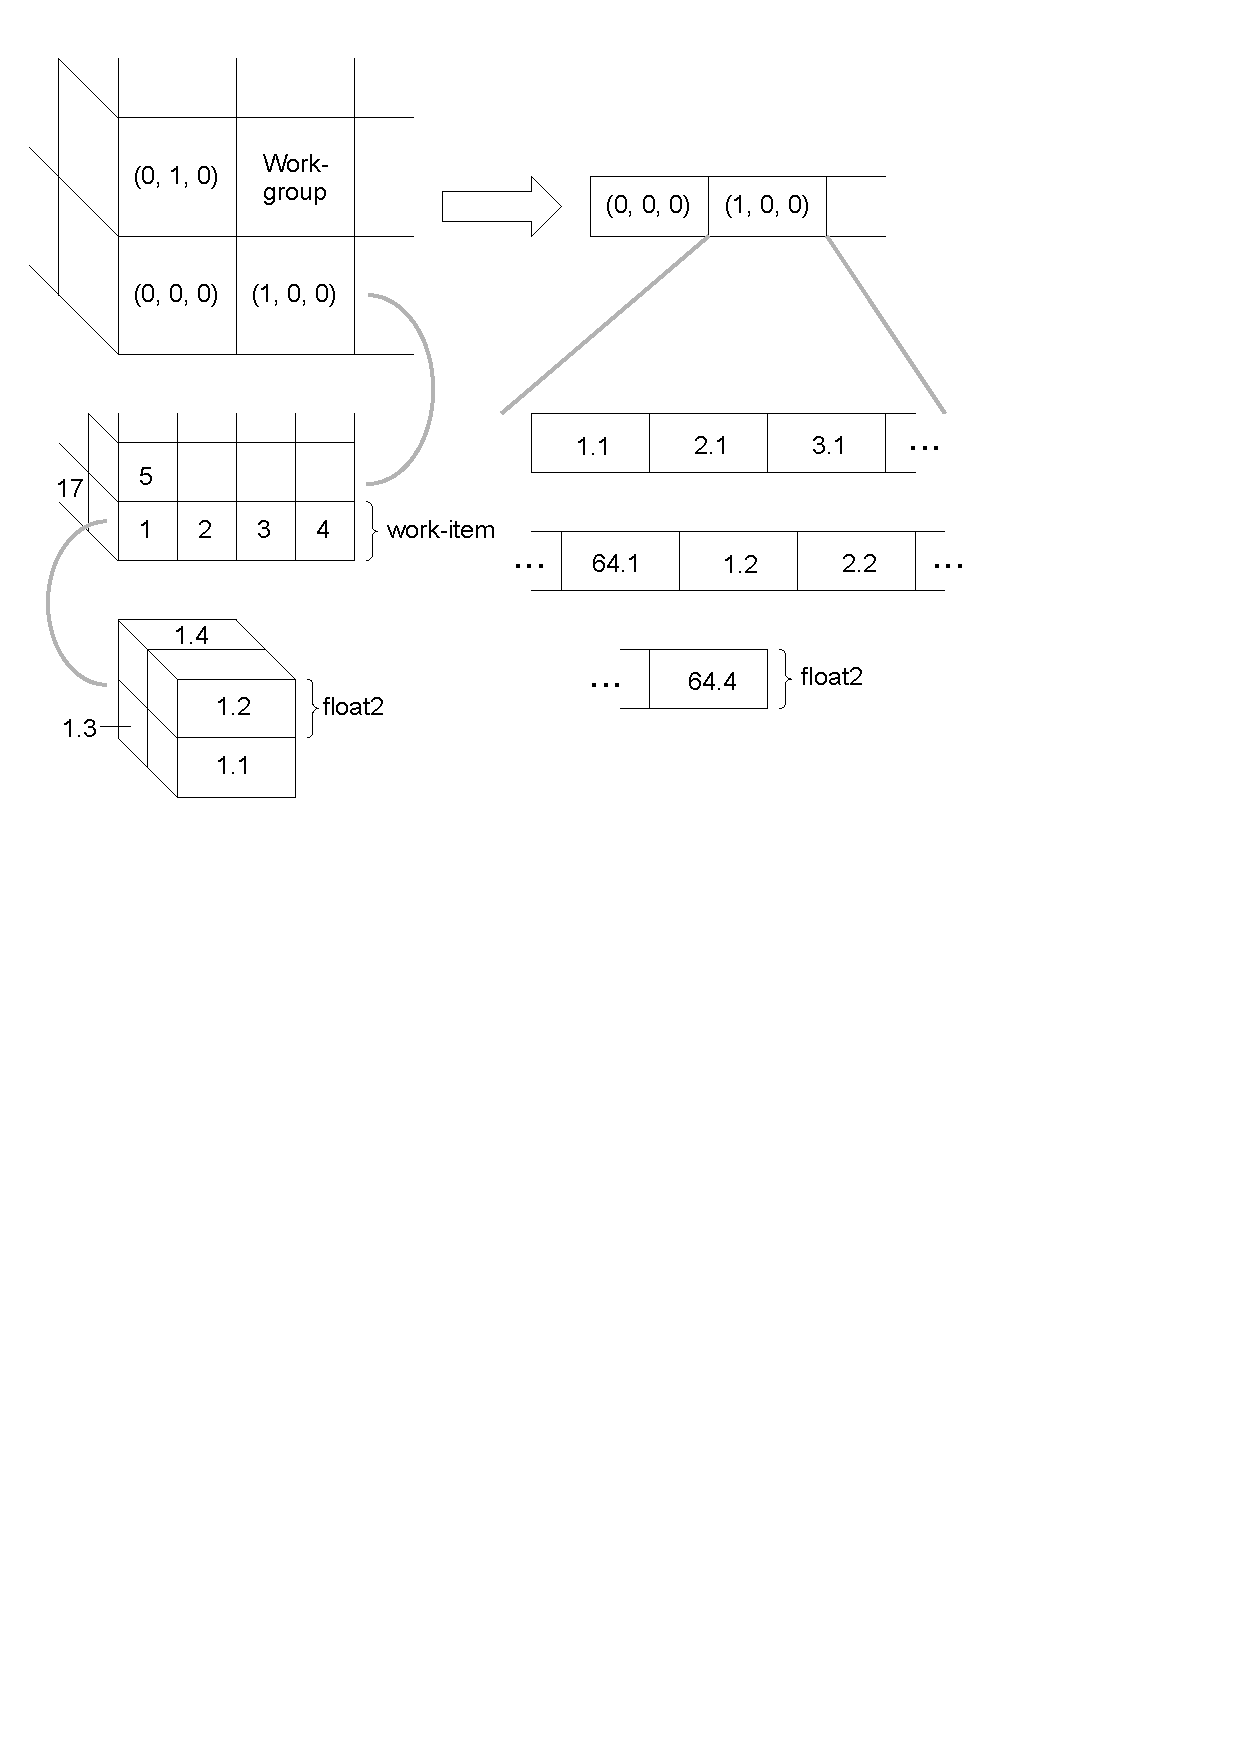
\includegraphics[width=\textwidth, trim=0 16cm 4cm 0, clip]{remap8}
\caption{\label{remap8}Schikking van \TT{} voor float8x8x8 met aaneengesloten blokken.}
\end{figure}

\subsubsection{Impact op de code}
Omdat de elementen van \TT{} op een andere plaats staan, moeten nu op een andere manier rondspringen. Voor deze herschikking moeten we elke iteratie gewoon 64 stappen vooruit springen. De beginplaatsen berekenen we als volgt. We bepalen eerst in welke blok de gegevens voor de work-group zit en berekenen het adres voor het eerste element van die blok. Vervolgens tellen we het volgnummer van het work-item op bij dit adres. De aangepaste kernel noemen we float8x8x8R. (float8x8x8 Remapped) De volledige broncode is beschikbaar appendix \refCode{float8x8x8R}. De code van float16x16x16R is beschikbaar in appendix \refCode{float16x16x16R}. De aanpassingen voor float8x8x8 zijn de volgende:
\begin{lstlisting}
//Old
int gId1 = get_global_id(0);
int gId2 = get_global_id(1);
int gId3 = get_global_id(2);

int jumpIdxTMode2 = I1;
int jumpIdxTMode3 = 2*I1*I2;

int idxT = gId1 + 
	2*gId2 * jumpIdxTMode2 +
	2*gId3 * jumpIdxTMode3;

int jumpNextIdxTMode2 = jumpIdxTMode2;
int jumpNextIdxTMode3 = jumpIdxTMode3 - 2*jumpIdxTMode2;

float2 sum2 = 0;

#pragma unroll
for(int i1 = 0, j = 0; i1 < 2; i1++)
{
	#pragma unroll
	for(int i2 = 0; i2 < 2; i2++, j++)
	{
		temp = c[j] - T[idxT];
		sum2 += temp*temp;
		
		idxT += jumpNextIdxTMode2;
	}
	idxT += jumpNextIdxTMode3;
}

//New
int lIdx = get_local_id(0) + 4 * get_local_id(1) + 16 * get_local_id(2);
int gIdx = get_group_id(0) + get_num_groups(0) * (get_group_id(1) + get_num_groups(1) * get_group_id(2));

int idxT =  lIdx + 256 * gIdx;   

float2 sum2 = 0;

#pragma unroll
for(int i = 0; i < 4; i++)
{
	temp = c[j] - T[idxT];
	sum2 += temp*temp;
		
	idxT += 64;
}
\end{lstlisting}
Bij het berekenen van de som verwijderen we de volgende twee lijnen omdat we die al berekenend hebben vlak voor de T-lus.
\begin{lstlisting}
int lIdx = get_local_id(0) + 4 * get_local_id(1) + 16 * get_local_id(2);
...
int gIdx = get_group_id(0) + get_num_groups(0) * (get_group_id(1) + get_num_groups(1) * get_group_id(2));
\end{lstlisting}

\subsubsection{Herschikking}
We moeten de elementen van \TT{} eerst herschikken. Net als bij de berekening van $f$ gaan we work-item laten overeenkomen met een 2x2x2 blok in \TT{}. De kernel die \TT{} herschikt bestaat gewoon uit een T-lus. Deze T-lus is een samensmelting van de T-lussen van float8x8x8 en float8x8x8R.

We berekenen eerst het beginpunt en de sprongafstanden in \TT{}. We berekenen ook het beginpunt in het herschikte geheugen.
Deze berekeningen zijn identiek aan de berekeningen in float8x8x8 en float8x8x8R. Dan gaan we in de T-lus elk element herschikken.

De kernel die \TT{} herschikt noemen we float8x8x8Mapper. De broncode voor float8x8x8Mapper en float16x16x16Mapper kan men terugvinden in appendices \refCode{float8x8x8Mapper} en \refCode{float16x16x16Mapper}.

\subsection{Isoleren van geheugenaanvragen}
We stellen ook een tweede herschikking voor. Het doel is dat alle work-items slechts \'e\'en kanaal gebruiken. We gaan dit toepassen op float16x16x16, maar we kunnen dit met enkele aanpassingen ook gebruiken voor andere kernels. De aangepaste float16x16x16 kernel noemen we float16x16x16I (float16x16x16 Isolated).

Een kanaal is 256 B breed. Dat zijn 16 float4's. Dit is gelijk aan het aantal float4's dat een work-item verwerkt. We gaan een strook van 16 float4's voorzien voor elke work-item. De eerste 256 B van het geheugen wijzen we toe aan het eerste work-item van de eerste work-group. De volgende 256B bevinden zich op het volgende kanaal en zijn dus voor het eerste work-item van de tweede work-group. Nadat er acht kanalen en acht work-groups gepasseerd zijn, is het de beurt aan het tweede work-item van de eerste work-group. Deze zit in hetzelfde kanaal als het eerste work-item maar wel in een andere bank.

De volgende vraag die we ons stellen is waar we het eerste work-item van de negende work-group moeten opslaan. De negende work-group is pas aan de beurt wanneer alle work-items van alle acht work-items geplaatst zijn. We noemen een groep van acht work-items een acht-groep. Een acht-groep bevat $16 * 16 * 16 * 8$ = 32Ki floats. Dit zijn 8192 float4's.

We delen dus het geheugen op in blokken van 8192 float4's lang. Deze blokken noemen we een acht-groepblok. Het geheugen in de acht-groepblok is toegewezen aan een acht-groep dat bestaat uit acht work-groups. De acht-groepblok is verdeeld in stroken die elk 16 float4's lang zijn. We noemen dit een kanaalstrook. Alle kanaalstroken binnen dezelfde acht-groepblok die bediend worden door hetzelfde kanaal vormen een kanaalblok. We wijzen de kanaalblokken toe aan de work-groups. Elke kanaalstrook wordt toegewezen aan een work-item binnen de work-group. Deze concepten worden ge\"illustreerd in figuur \ref{iso}.

\begin{figure}
\centering
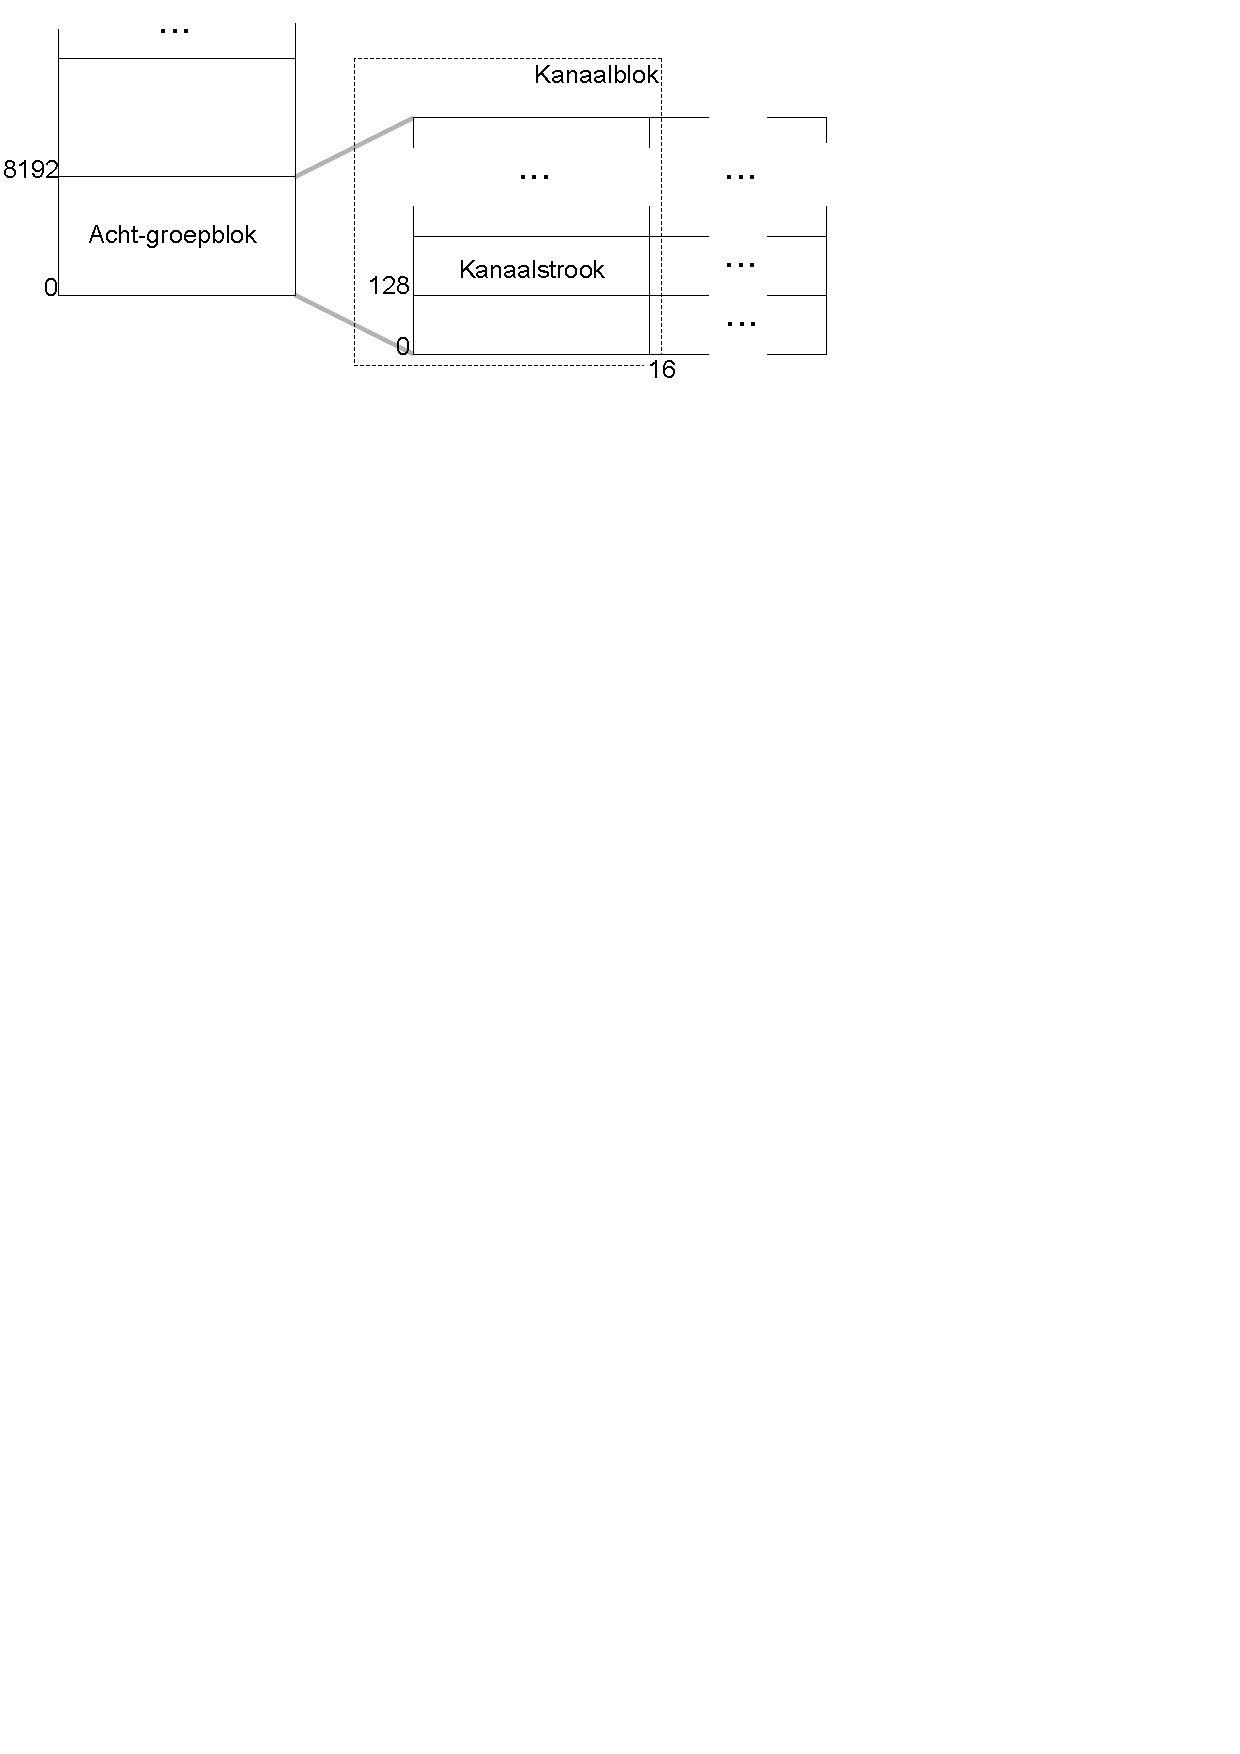
\includegraphics[trim=0 23cm 6.5cm 0, clip]{iso}
\caption{\label{iso}Onderverdeling van het geheugen bij een herschikking zonder kanaalconflicten.}
\end{figure}

Voor een willekeurig work-item bepalen we de beginplaats als volgt :
\begin{itemize}
    \item Lineariseer het volgnummer van de work-groep en deel dit getal door acht. Rond dit getal af naar beneden. Dit bepaalt in welke acht-groep het work-item zit. Vermenigvuldig het afgeronde getal met 8192. Dit is het beginadres van de acht-groepblok.
    \item Bepaal het kanaal waarin de work-group thuis hoort. Dit is gelijk aan het gelineariseerde volgnummer van de work-groep modulo acht. Vermenigvuldig dit getal met 16 en tel dit op bij het beginadres van de acht-groepblok. We zitten nu in de juiste kanaalblok. We noemen dit het beginadres van de kanaalblok.
    \item Lineariseer het volgnummer van de work-item binnen de work-groep en vermenigvuldig dit met 128. Tel dit getal op bij het beginadres van de kanaalblok. We zitten nu in het beginadres van de kanaalstrook die toegewezen is aan het work-item.
\end{itemize}

\subsubsection{Impact op de code}
We gaan vertrekken vanuit float16x16x16R en niet vanuit float16x16x16. We doen dit omdat  float16x16x16I meer gemeenschappelijk heeft met  float16x16x16R dan met float16x16x16. De aanpassingen die we aan float16x16x16R doen zijn identiek dezelfde als de aanpassingen die we aan float16x16x16Mapper moeten doen om float16x16x16MapperI te krijgen. Zie \refCode{float16x16x16I} en \refCode{float16x16x16MapperI} voor de broncode voor respectievelijk float16x16x16I en float16x16x16MapperI.

\begin{lstlisting}
//Old
int idxT =  lIdx + 1024 * gIdx;
...
#pragma unroll
for(int i = 0; i < 16; i++)
{
	...
	idxT += 64;
}

//New
int channel = gIdx % 8;

int idxT =  8192 * (gIdx/8) + 16*channel + 128*lIdx; 
...
#pragma unroll
for(int i = 0; i < 16; i++)
{
	...
	idxT++;
}
\end{lstlisting}

\section{Geschiktheid gradi\"ent}
We herhalen nog eens hoe we de gradi\"ent van een derde-orde tensor berekenen:
\begin{align*}
    g^{(1)}_{ir} =& \sum_{j'}^{I_2}\sum_{k'}^{I_3} f_{ij'k'} u^{(2)}_{j'r} u^{(3)}_{k'r}\\
    g^{(2)}_{jr} =& \sum_{i'}^{I_1}\sum_{k'}^{I_3} f_{i'jk'} u^{(1)}_{i'r} u^{(3)}_{k'r}\\
    g^{(3)}_{kr} =& \sum_{i'}^{I_1}\sum_{j'}^{I_2} f_{i'j'k} u^{(1)}_{i'r} u^{(2)}_{j'r}\\
\end{align*}

We gaan nu de rekenverhouding berekenen. We veronderstellen hierbij dat \FF{} al berekend is.

\begin{tabular}{|r l|c| c|c|}
\hline
					&			& flop(sp)			& flop(dp) 			& \# geh. aanvragen	\\
\hline
$a_{j'k'r}$	&$= u^{(2)}_{j'r} u^{(3)}_{k'r}$%
								& $2 R \cdot I^2$	& $2 R I^2$			&	$2 R I$			\\
$a_{i'j'k'r}$	&$= f_{ij'k'} \cdot a_{j'k'r}$%
								& $2 R I^3$			& $2 R I^3$			&	$I^3$			\\
$g^{(1)}_{ir}$	&$= \sum_{j'}^{I_2}\sum_{k'}^{I_3}a_{i'j'k'r}$%
								& 0 (MAD)			& 0 (MAD)			&	$R I$			\\
\hline
\end{tabular}

De rekenverhouding is gelijk aan:
\[
	\frac{2R(I^3 + I^2)}{I^3 + 3RI}
\]

Voor hoge waarden van $I$ convergeert de rekenverhouding naar $2R$. Dit is ook zichtbaar wanneer we de rekenverhouding plotten in functie van $R$ en $I$. Zie figuur \ref{haalG}.

\begin{figure}
\centering
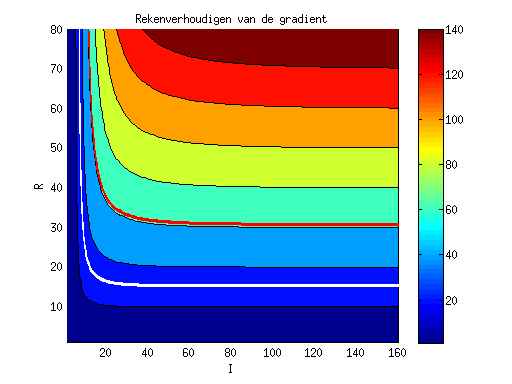
\includegraphics{haalG}
\caption{\label{haalG}De rekenverhoudingen van de gradi"ent. Het kantelpunt voor de GPU met enkele precisie is getekend met een rode lijn. Het kantelpunt voor dubbele precisie is getekend met een witte lijn.}
\end{figure}

Wanneer we \ref{haalG} naast \ref{haalF} leggen zien we dat beide grafieken bijna identiek zijn. Laten we de rekenverhouding van $f(\T, \mUUU)$ eens aftrekken van de rekenverhouding van de gradi"ent.
\begin{align*}
		&	\frac{2R (I^3 + I^2) + 2I^3}{I^3 + 3RI} - \frac{2R (I^2 + I^3)}{3RI + I^3}\\
		=&	\frac{2R(I^3 + I^2) + 2I^3 - 2R (I^2 + I^3)}{I^3 + 3RI}\\
		=&	\frac{2I^3}{I^3 + 3RI}\\
\approx  &	2
\end{align*}
We besluiten hieruit dat de rekenverhoudingen van de gradi"ent twee flop(sp)/float en twee flop(dp)/double lager liggen dan de rekenverhoudingen van $f(\T, \mUUU)$. Twee  is klein tegenover 61,43 flop(sp)/float en 30,71 flop(dp)/double. Daarom zeggen we dat het geschikt is om de gradi"ent uit te voeren op de grafische als en slechts als het geschikt is om $f(\T, \mUUU)$ uit te voeren op de grafische kaart.

\subsection{\FF{} berekenen}
We gingen er vanuit dat \FF{} gegeven was. \FF{} is een neveneffect van het berekenen van $f$. We kunnen elke kernel die $f$ berekent aanpassen om ook \FF{} weg te schrijven. Door deze aanpassing verandert ook de rekenverhouding.

De rekenverhouding voor een onaangepaste kernel is gelijk aan:
\[
    \frac{2R (I^2 + I^3) + 2I^3}{3RI + I^3}
\]

We gaan $I^3$ extra getallen wegschrijven. Hierdoor verandert de rekenverhouding naar:
\[
    \frac{2R (I^2 + I^3) + 2I^3}{3RI + 2I^3}
\]
Als $I$ groot genoeg is kunnen we de rekenverhouding benaderen met $R + 1$.  Dit is een halvering tegenover de rekenverhouding van $f(\T, \mUUU)$ en dat is ook zichtbaar in figuur \ref{haalFG}. We zeggen dat de aangepaste versie van $f(\T, \mUUU)$ geschikt is om uit te voeren op de grafische kaart als en slechts de onaangepaste versie $f(\T, \mUUU)$ geschikt is om uit te voeren op de grafische kaart met een rang die gelijk is aan de helft van de rang van de aangepaste versie.

\begin{figure}
\centering
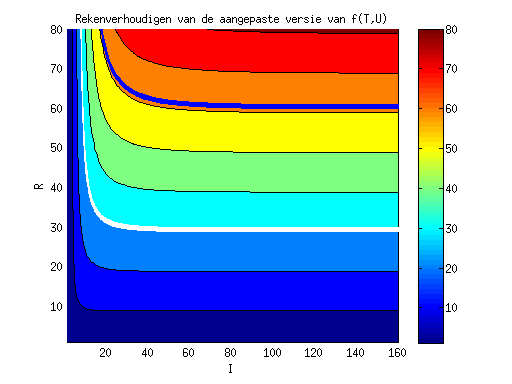
\includegraphics{haalFG}
\caption{\label{haalFG}De rekenverhoudingen van de aangepaste versie van $f(\T, \mUUU)$. Het kantelpunt voor de GPU met enkele precisie is getekend met een blauwe lijn. Het kantelpunt voor dubbele precisie is getekend met een witte lijn.}
\end{figure}

\section{Gradi\"ent-kernel}
Alle voorgaande kernels gebruikten we float's, maar we hebben wel alle berekeningen ook voor doubles gedaan. Daarom gaan we voor de gradi"ent met doubles werken. We kunnen alle float-kernels omvormen naar doubles door het sleutelwoord ``float'' te vervangen door ``double''.

\section{Double16x16x16FG}
Als eerste gaan we double16x16x16 aanpassen naar double16x16x16FG. Het verschil er tussen is dat double16x16x16FG ook \FF{} wegschrijft. Dit is een eenvoudige aanpassing:
\begin{lstlisting}
//Old
..., __global double* sum)
{
	...
	temp = c[j] - T[idxT];
	sum4 += temp*temp;

//New
..., __global double* sum, __global double4* F)
{
	...
	temp = c[j] - T[idxT];
	F[idxT] = temp;
	sum4 += temp*temp;
\end{lstlisting}

De volledige broncode is beschikbaar in appendix \refCode{double16x16x16FG}.

\section{De gradi"ent-kernel}
We gaan voor deze kernel een 2DRange gebruiken. E\'en dimensie voor $r$ en \'e\'en dimensie voor $i$, $j$ of $k$. We noemen de kernel ``double16x16G'' (double16x16 Gradient) omdat de kernel de gradi\"ent berekent waarbij elke work-group overeenkomt met een $16 \times 16$ blokje in de gradi\"entmatrix. Een work-item komt overeen met een $2 \times 2$ blokje. Er zijn in totaal dus 64 work-items.

We associ\"eren de eerste dimensie van de 2DRange met $r$. Hierdoor zal de GPU eerst work-groups activeren met dezelfde waarde voor $i$. (of $j$ of $k$) Omdat alle work-items elkaar achter de hielen lopen zullen ze vlak na elkaar dezelfde $f_ij'k'$ (of $f_i'jk'$ of $f_i'j'k$) ophalen. Hierdoor kunnen de caches optimaal werken.

We kunnen de gradi"ent berekenen met een eenvoudig algoritme. We geven hieronder zo een algoritme in pseudo-code. Het algoritme berekent enkel elementen uit de eerste gradi\"entmatrix. De algoritmes voor de andere twee gradi\"entmatrices zijn varianten op het algoritme voor de eerste gradi\"entmatrix.
\begin{lstlisting}
Gradient(indexMode1, R):
	sum = 0
	foreach indexMode2 in [1:I2]:
		foreach indexMode3 in [1:I3]:
			sum += 	F[indexMode1, indexMode2, indexMode3] *
					U2[indexMode2, R] *
					U3[indexMode3, R]
	G[indexMode1, R] = sum
\end{lstlisting}

Het nadeel van bovenstaand algoritme is dat de elementen van \UU{2} en \UU{3} beiden $I_2$ * $I_3$ keer gelezen worden. We kunnen dit optimaliseren door het element van \UU{2} buiten de tweede lus in te lezen.

\begin{lstlisting}
Gradient(indexMode1, R):
	sum = 0
	foreach indexMode2 in [1:I2]:
		u2 = U2[indexMode2, R]
		foreach indexMode3 in [1:I3]:
			sum += 	F[indexMode1, indexMode2, indexMode3] *
					u2 * U3[indexMode3, R]
	G[indexMode1, R] = sum
\end{lstlisting}

We lezen elk element van \UU{2} nu maar \'e\'en maal in. Maar de elementen van \UU{3} lezen we nog steeds $I_2$ keer in.
We lossen dit op door de elementen van \UU{3} te cachen. De cache is 64 elementen groot, waardoor elk element van $I_3$ maar eenmaal gelezen worden. De elementen van \UU{2} worden nu $I_3/64$ keer gelezen.

De 64 double in de cache nemen over de hele work-group 32KiB van het registergeheugen in. Dit past acht maal in het registergeheugen. Stel dat we de cache delen in het lokaal geheugen. We hebben dan acht caches van 64 doubles nodig. Dit neemt 4 KiB in. Er is maar 32KiB lokaal geheugen beschikbaar. Dit beperkt het aantal work-items ook tot acht. We kiezen toch voor het registergeheugen omdat we bij het lokaal geheugen extra cycli verliezen met de geheugeninstructies.

De pseudo-code:

\begin{lstlisting}
Gradient(indexMode1, R):
	sum = 0
	while elementsLeftInMode3():
		cacheNext64ElementOfU3()
		
		foreach indexMode2 in [1:I2]:
			u2 = U2[indexMode2, R]
			foreach cachedU3Element in cache:
				sum += 	F[indexMode1, indexMode2, indexMode3] *
						u2 * cachedU3Element
	G[indexMode1, R] = sum

elementsLeftInMode3():
	return indexMode3 < I3

cacheNext64ElementOfU3():
	clear(cache)
	while elementsLeftInMode3():
		append(cache, U3[indexMode3, R])
\end{lstlisting}

\section{Besluit}
We hebben voor het berekenen van de doelfunctie en de gradi\"ent onderzocht of ze de volledige rekenkracht van de grafische kaart wel kunnen benutten. We hebben aangetoond dat de rekenverhouding onder bepaalde realistische omstandigen hoog genoeg is om de volledige rekenkracht te kunnen benutten.

Voor het berekenen van de doelfunctie hebben we vijf varianten ontwikkeld: float16x16x16, float16x16x16R, float16x16x16I, float8x8x8 en float8x8x8R. De varianten die eindigen op R en op I zijn varianten die het globaal geheugen effici\"enter gebruiken. De 8 en 16 in de naam geven aan hoeveel element een work-group verwerkt. Bij float16x16x16 verwerkt een work-group een blokje van 16$\times$16$\times$16 elementen met enkele precisie.

Voor het berekenen van de gradi\"ent van de doelfunctie hebben we maar \'e\'en kernel ontwikkeld die in dubbele precisie werkt. Deze kernel verwacht dat de kernel die de doelfunctie berekent ook enkele tussenresultaten wegschrijft. We hebben daarom nog een extra variant voor het berekenen van de doelfunctie ontwikkeld.